\documentclass[12pt]{article}
\usepackage[utf8]{inputenc}
\usepackage[T2A]{fontenc}
\usepackage[russian]{babel}
\usepackage{amsmath}
\usepackage{amssymb}
\usepackage{dsfont}
\usepackage[dvipsnames]{xcolor}
\usepackage{setspace}
\usepackage{multirow}
\usepackage[a4paper, outer=1.5cm, inner=1.5cm, top=1cm, bottom=1cm]{geometry}
\usepackage{graphicx}
\usepackage{skull}
\usepackage{wasysym}
\usepackage{float}
\graphicspath{{.images/}}
\usepackage{hyperref}
\hypersetup{colorlinks=true, linkcolor=blue, filecolor=magenta, urlcolor=cyan}
\usepackage[firstpage]{draftwatermark}
\SetWatermarkText{
    $\qquad\qquad\qquad\qquad\qquad$\parbox{7cm}{\begin{center}
    
\includegraphics[width = 0.08\textwidth]{lion-logo.png}\bigskip\\~\bigskip\\~\vspace{-24mm}\\~\end{center}}
}
\SetWatermarkAngle{0}
\SetWatermarkScale{1.5}
\usepackage{etoolbox}

\newtoggle{ifsolved}
\newtoggle{needhelp}
\newcounter{num}
\setcounter{num}{1}

\newcommand{\newnum}{\par\textbf{\textnumero\arabic{num}}\stepcounter{num}}
\newcommand{\sol}{\vspace{3mm}\par\textbf{Решение: }}
\newcommand{\ans}{\vspace{3mm}\par\textbf{Ответ: }}
\newcommand{\hint}{\vspace{3mm}\par\textbf{Подсказка: }}
\newcommand{\mode}[1]{
\ifstrequal{#1}{0}{\togglefalse{ifsolved}\togglefalse{needhelp}}{\ifstrequal{#1}{1}{\togglefalse{ifsolved}\toggletrue{needhelp}}{\ifstrequal{#1}{2}{\toggletrue{ifsolved}\togglefalse{needhelp}}{\toggletrue{ifsolved}\toggletrue{needhelp}}}}} %if 0 - if 1 - if 2 - else
%\newenvironment{problem}[8]{%#1, #2, #3
%\parbox{\linewidth}{\vspace{4mm}\ifstrequal{#4}{(лёгкая)}{\newnum\textbf{.}}{\newnum\textbf{*.} } \\ #5}
%\iftoggle{ifsolved}{\sol #6}{}
%\iftoggle{ifsolved}{\ans #7}{}
%\iftoggle{needhelp}{\hint #8}{}}

\newenvironment{problem}[8]{%#1, #2, #3
\parbox{\linewidth}{\vspace{5mm}\ifstrequal{#4}{(лёгкая)}{\newnum\textbf{.}}{\newnum\textbf{*.} } \\ #5}
\iftoggle{ifsolved}{\sol #6}{}

\iftoggle{ifsolved}{\parbox{\linewidth}{\ans #7}}{}
\iftoggle{needhelp}{\parbox{\linewidth}{\hint #8}}{}}

\newenvironment{mylist} %custom list
{ \begin{itemize}
    \setlength{\itemsep}{0pt}
    \setlength{\parskip}{0pt}
    \setlength{\parsep}{0pt}     }
{ \end{itemize}                  }

\newenvironment{homeass}[1]{\vspace*{-1.5cm}
\iftoggle{ifsolved}{
    \section*{\center{Решение домашнего задания к #1.}}
}{
    \section*{\center{\textcolor{Sepia}{Домашнее задание к #1}}}
} \vspace{7mm}\large}

\parindent=0pt
\pagestyle{empty}
%$\!$[\arabic{class}.\arabic{num}]
%\ifnumcomp{\value{counter}}{>}{1}{true}{false}
%\definecolor{Gray}{gray}{0.9}
%\definecolor{mypink}{RGB}{219, 48, 122}
%\newcolumntype{g}{>{\columncolor{Gray}}p{2.8cm}}

\begin{document}
\large
\mode{7}
%0 for problems without hints
%1 for problems + hints
%2 for problems + solutions + answers
%else: show all

{\centering\section*{СПИСОК ЗАДАЧ}}

{\centering\subsection*{\smallskip\\\textcolor{green}{\textbf{Полезные вещи, которые можно и нужно копипастить:}}}}

\subsection*{\textcolor{Emerald}{\textbf{Полезные шпаргалки по LaTeXу:}}}

\textbf{Пример вставки рисунка:}

\begin{minipage}{\linewidth}
    \begin{minipage}{0.54\linewidth}
    см. рисунок справа\\
    Текст к собственно пикче, примерно всегда это либо развёрнутое описание, либо большая часть решения задачи --- стремимся экономить пространство, если это можно сделать.
    \end{minipage}
    \hspace{0.05\linewidth}
    \begin{minipage}{0.4\linewidth}
    \begin{figure}[H] 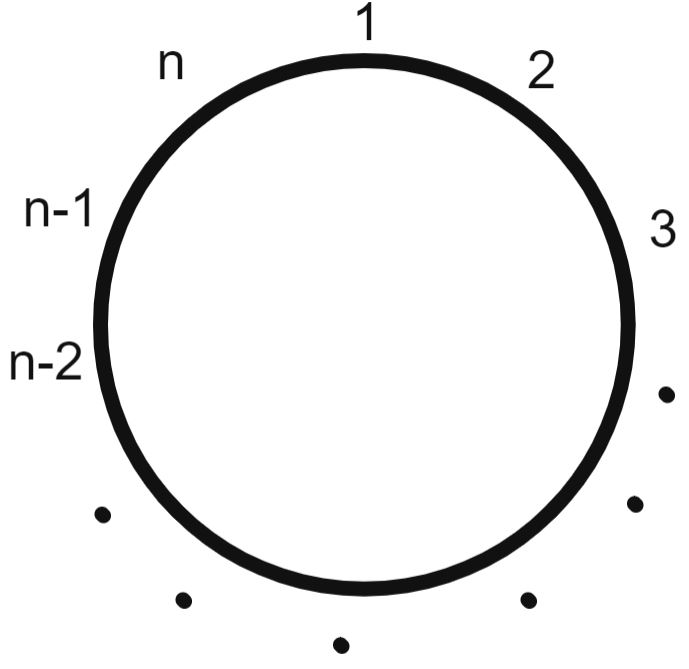
\includegraphics[width=\linewidth]{sol3} %тут поменять имя пикчи
    \end{figure}
    \end{minipage}
\end{minipage}

\textbf{Дефолтные математические знаки и символы:}\\
$\geqslant$,
$\leqslant$,
$a^{b}$,
$x_{i}$,
$\sqrt{a}$,
$\frac{a}{b}$,
$\displaystyle \frac{a}{b}$,
$\cdot$
$\;\Rightarrow\;$,
$\;\Leftrightarrow\;$,
$1{,}2$.
О промежутках:
$a\!b$,
$a\,b$,
$a\:b$,
$a\;b$,
$a\quad b$.

\textbf{Стандартные система и совокупность уравнений / неравенств:}\\
$\left\{
\begin{aligned}
f(x) &= 0 \\
g(x) &= 1
\end{aligned}\right.$

$\left[\begin{aligned}
&\left\{\begin{aligned}
f(x) &\geqslant a \\
g(x) &= b
\end{aligned}\right.\\
&\left\{\begin{aligned}
f(x) &< a \\
g(x) &= -b
\end{aligned}\right.
\end{aligned}\right.$

\subsection*{\textcolor{Emerald}{\textbf{Не математическое, но полезное:}}}
% комментарий в любом месте документа, который нигде не будет видно. Можно использовать для написания заметок-вопросов по задачам
\textbf{Пример таблицы:}

\begin{tabular}{|c|c|c|}
\hline
    $a$ & $b$ & текст
\\\hline
    $c$ & $d$ & мораль
\\\hline
\end{tabular}\\

\textbf{Отступы:} между\smallskip\\ строками\medskip\\ \textbf{Тире} --- это три дефиса.\\
\textbf{Списки:}
\begin{mylist}
\item [$\bullet$] это был пункт а
\item [2)] а это уже пункт номер 2 с изменённым заголовком
\end{mylist}

\subsection*{\textcolor{Emerald}{\textbf{Всё, неупомянутое выше (или если просто что-то не так):}}}
\begin{mylist}
\item [$\bullet$] Решение отдельных вопросов касательно ТеХа нужно искать в \href{https://www.mccme.ru/free-books/llang/newllang.pdf}{Львовском}.

\item [$\bullet$] Найти произвольный символ, который нужен, можно в \href{http://detexify.kirelabs.org/classify.html}{Detexify}.

\item [$\bullet$] Если возникли сомнения при решении, ответ практически ко всем задачам можно проверить с помощью \href{https://www.wolframalpha.com/}{WolframAlpha}.

\item [$\bullet$] Если в задаче нужно создать картинку, то лучше пока отложить эту задачу. Все графики планируется централизованно нарисовать (или перерисовать) в геогебре.

\item [\textcolor{brown}{\textbf{!!}}] Важно ставить \textcolor{red}{\textbf{$\spadesuit$}}
(или просто red) в тело задачи в случае серьёзных вопросов к решению и какой-то вопиющей лажи.

\item [\textcolor{brown}{\textbf{!!}}] Важно ставить \textcolor{olive}{\textbf{$\spadesuit$}}
(или просто olive) в тело задачи в случае не самого удачного текста и кривых отступов.
\end{mylist}

\subsection*{\textcolor{Violet}{\textbf{Комментарии:}}}% а также невидимые комментарии - так можно оставлять заметки-вопросы прямо в задаче, чтобы потом было понятно, в чём вопрос.
\begin{mylist}
\item [$\skull$] Переставлять задачи местами --- очень плохая идея.

\item [$\smiley$] При двойном клике по тексту pdf справа происходит автоматический переход к этому месту в латех-коде, а для обратного перехода можно нажать стрелку вправо (висит сверху между pdf и латех-кодом).

\item [$\smiley$] Если есть размышления, дописывать red/olive к задаче или не дописывать, то лучше всё-таки дописать.

\item [$\skull$] Самое плохое, что можно сделать --- написать в любое поле из трёх (НаписанноеРешение/ВерныйОтвет/Подсказка) только половину того, что надо, никак это не отметить, и потом пойти дальше.\\ Нужно в этот момент писать red/olive в случайном месте задачи, чтобы потом вычислить это с помощью Ctrl+F по всему документу (и это то, что потом будет делаться долго и тщательно)
\end{mylist}

\newpage
\setcounter{num}{1502}

\hypertarget{10.4}{{\centering\section*{\bigskip\\\textcolor{Blue}{\hyperlink{start2}{\textcolor{Blue}{10.4}} Преобразование тригонометрических выражений.}\vspace{-5mm}}}}

\begin{problem}{Синус и косинус суммы и разности аргументов.}{10.4.1}{9D}{(лёгкая)}
{Убедиться, что теорема Пифагора выполнена для угла $\alpha + \beta$, то есть, используя формулы для синуса и косинуса суммы, проверить, что верно равенство\\ $\sin^{2}(\alpha + \beta) + \cos^{2}(\alpha + \beta) = 1$.}
{НаписанноеРешение}
{ВерныйОтвет}{Подсказка}
\end{problem}

\begin{problem}{Тангенс суммы и разности аргументов.}{10.4.2}{9D}{(лёгкая)}
{Используя формулы для косинуса и синуса суммы, вывести формулу для тангенса суммы и показать что $\,\displaystyle \tg(\alpha + \beta) = \frac{\tg \alpha + \tg \beta}{1 - \tg \alpha \tg \beta}$.}
{НаписанноеРешение}
{ВерныйОтвет}{Подсказка}
\end{problem}

\begin{problem}{Формулы приведения.}{10.4.3}{9D red многопунктовая}{(лёгкая)}
{Выписать формулу, показывающую, как связаны синусы и косинусы углов
\\a) для диаметрально противоположных точек;
\\b) для точек, получаемых друг из друга поворотом на 90$^{\circ}$ против часовой стрелки;
\\с) для точек, получаемых друг из друга поворотом на 90$^{\circ}$ по часовой стрелке.}
{НаписанноеРешение}
{ВерныйОтвет}{Подсказка}
\end{problem}

\begin{problem}{Формулы приведения.}{10.4.3}{9D}{(лёгкая)}
{Найти значение выражения $\,\displaystyle \sin 23^{\circ} - \cos 67^{\circ}$.}
{Можно заметить, что $67^{\circ} + 23^{\circ} = 90^{\circ}$. Получается, что $\sin 67^{\circ} = \cos 23^{\circ}$ и наоборот, $\cos 67^{\circ} = \sin 23^{\circ}$. Таким образом, данное выражение равно нулю.}
{$\,\displaystyle \sin 23^{\circ} - \cos 67^{\circ} = 0$.}{$23^{\circ} + 67^{\circ} = 90^{\circ}$.}
\end{problem}

\begin{problem}{Формулы приведения.}{10.4.3}{9D}{(лёгкая)}
{Найти значение выражения $\,\displaystyle \frac{5\sin 61^{\circ}}{\sin 299^{\circ}}$.}
{Можно заметить, что $61^{\circ} + 299^{\circ} = 360^{\circ}$.\\ Это означает, что здесь можно воспользоваться формулой приведения (или нарисовать оба угла и увидеть равные треугольники). В итоге получается, что $\sin 299^{\circ} = - \sin 61^{\circ}$ (треугольники симметричны относительно оси абсцисс).\\ Таким образом, $\,\displaystyle \frac{5\sin 61^{\circ}}{\sin 299^{\circ}} = \frac{5\sin 61^{\circ}}{-\sin 61^{\circ}} = -5$ (так как $\sin 61^{\circ} \neq 0$).}
{$\,\displaystyle \frac{5\sin 61^{\circ}}{\sin 299^{\circ}} = -5$.}{Используй формулы приведения.}
\end{problem}

\begin{problem}{Формулы приведения.}{10.4.3}{9D}{(лёгкая)}
{Найти значение выражения $\,\displaystyle \sin 12^{\circ} + \sin 168^{\circ} + 2\cos 102^{\circ}$.}
{\vspace{-4mm}\\\begin{minipage}{\linewidth}
    \begin{minipage}{0.65\linewidth}
    ~\vspace{1mm}\\
    Можно заметить, что все углы в этом выражении связаны: $12^{\circ} + 168^{\circ} = 180^{\circ}$, $102^{\circ} = 12^{\circ} + 90^{\circ}$.\smallskip\\ Поэтому, если вспомнить формулы приведения, или изобразить эти углы явно (см. рисунок справа), становится очевидно, что $\sin 168^{\circ} = \sin 12^{\circ}$ и что $\cos 102^{\circ} = - \sin 12^{\circ}$. Поэтому $\sin 12^{\circ} + \sin 168^{\circ} + 2\cos 102^{\circ} = \sin 12^{\circ} + \sin 12^{\circ} + 2 (-\sin 12^{\circ}) = 0$.
    \end{minipage}
    \hspace{0.05\linewidth}
    \begin{minipage}{0.3\linewidth}\begin{figure}[H] 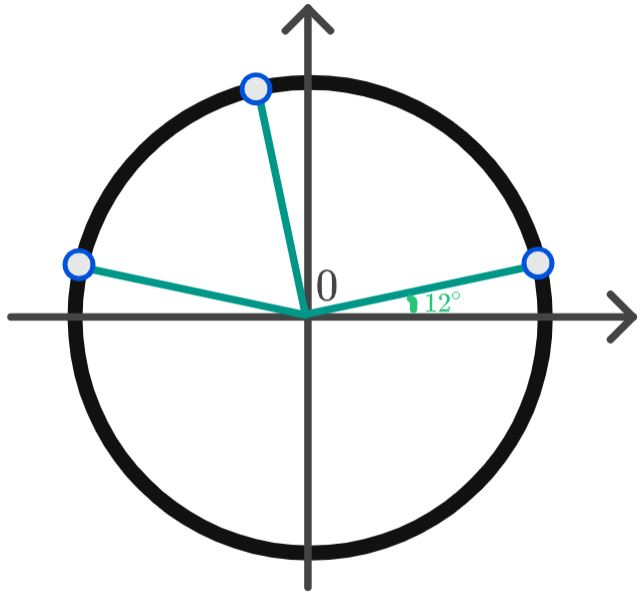
\includegraphics[width=\linewidth]{sol38}\end{figure}\end{minipage}
\end{minipage}\vspace{-2mm}}
{$\,\displaystyle \sin 12^{\circ} + \sin 168^{\circ} + 2\cos 102^{\circ} = 0$.}{Используй формулы приведения: тут три одинаковых треугольника.}
\end{problem}

\begin{problem}{Формулы приведения.}{10.4.3}{9D}{*}
{Найти значение выражения $\,\displaystyle \frac{5}{\sin^2 298^{\circ} + \cos^2 118^{\circ}} + \frac{1}{0{,}2}$.}
{Выражение в знаменателе очень похоже на теорему Пифагора, однако пока углы разные, непонятно, правда ли это катеты из одного треугольника.\\ Присмотревшись, замечаем, что $298^{\circ} = 118^{\circ} + 180^{\circ}$.\\ Используем формулу приведения: $\sin (\alpha + 180^{\circ}) = - \sin \alpha \;\Rightarrow\; \sin 298^{\circ} = -\sin 118^{\circ}$. Следовательно,
$\displaystyle \:\frac{5}{\sin^2 298^{\circ} + \cos^2 118^{\circ}} + \frac{1}{0{,}2} = \frac{5}{(-\sin 118^{\circ})^2 + \cos^2 118^{\circ}} + \frac{1}{\frac15} = $ \\ $\displaystyle \frac{5}{\sin^2 118^{\circ} + \cos^2 118^{\circ}} + 5 = \frac51 + 5 = 10$.}
{$\,\displaystyle \frac{5}{\sin^2 298^{\circ} + \cos^2 118^{\circ}} + \frac{1}{0{,}2} = 10$.}{Используй формулу приведения и теорему Пифагора.}
\end{problem}

\begin{problem}{Формулы приведения.}{10.4.3}{9D}{(лёгкая)}
{Что можно сказать о чётности и нечётности тангенса и котангенса?}
{НаписанноеРешение}
{ВерныйОтвет}{Подсказка}
\end{problem}

\begin{problem}{Формулы приведения.}{10.4.3}{9D}{(лёгкая)}
{Как и для других тригонометрических функций, для тангенса и котангенса также имеются формулы приведения. Выписать их все.}
{НаписанноеРешение}
{ВерныйОтвет}{Подсказка}
\end{problem}

\begin{problem}{Формулы приведения.}{10.4.3}{9D}{(лёгкая)}
{Доказать тождество: $\;\displaystyle \frac{\sin(\pi - \alpha) - \ctg(\alpha - \frac{\pi}{2})}{1 + \cos(-\alpha)} = \tg(\pi + \alpha)$.}
{Используем формулы приведения для каждой из четырёх тригонометрических функций. $\sin(\pi - \alpha) = \sin\alpha$ (симметрия относительно оси ординат). $\cos(-\alpha) = \cos\alpha$ (косинус~--- чётная функция, отражение относительно оси абсцисс не меняет $x$-координату). $\tg(\pi + \alpha) = \tg\alpha$ (при центральной симметрии синус и косинус меняют знаки, но их отношение остаётся таким же). $\ctg(\alpha - \frac{\pi}{2}) = -\tg\alpha$ (при повороте на 90 градусов по часовой стрелке <<синус и косинус меняются местами>>, поэтому отношение становится равным обратной величине, причём с другим знаком).\\
Итого: $\;\displaystyle \frac{\sin(\pi - \alpha) - \ctg(\alpha - \frac{\pi}{2})}{1 + \cos(-\alpha)} = \tg(\pi + \alpha) \;\Leftrightarrow\; \frac{\sin\alpha - (-\tg\alpha)}{1 + \cos\alpha} = \tg\alpha$.\\
Но $\displaystyle \frac{\sin\alpha - (-\tg\alpha)}{1 + \cos\alpha} = \frac{\sin\alpha + \tg\alpha}{1 + \cos\alpha} = \frac{\sin\alpha\cos\alpha + \sin\alpha}{\cos\alpha \cdot (1 + \cos\alpha)} = \frac{\sin\alpha \cdot (\cos\alpha \!+\! 1)}{\cos\alpha \cdot (1 \!+\! \cos\alpha)} = \tg\alpha$.\smallskip\\
Строго говоря, при сокращении дроби надо проверить, что $\cos\alpha \neq -1$. Однако, так как в данном выражении участвуют и тангенсы, и котангенсы, $\alpha = \frac{\pi n}{2}$ не являются допустимыми значениями (иначе где-то бы получилось деление на 0).}
{Смотри рассуждения выше.}{Используй формулы приведения для всех тригонометрических функций, а затем сократи дробь.}
\end{problem}

\begin{problem}{Формулы двойного аргумента и формулы понижения степени.}{10.4.4}{9D}{(лёгкая)}
{Вычислить значение выражения $\;\displaystyle 2\sin\frac{\pi}{12}\cos\frac{\pi}{12}$.}
{НаписанноеРешение}
{ВерныйОтвет}{Подсказка}
\end{problem}

\begin{problem}{Формулы двойного аргумента и формулы понижения степени.}{10.4.4}{9D}{(лёгкая)}
{По памяти (!) выписать формулы:\\ $\sin 2\alpha = {?} $\hfill $\cos 2\alpha = {?}\phantom{\cos\alpha\cos\alpha - \sin\alpha\cos\alpha + 111\cos\alpha}$\\
$\sin (\alpha + \beta) = {?}$\hfill$\cos (\alpha + \beta) = {?}\phantom{\cos\alpha\cos\alpha - \sin\alpha\cos\alpha + 111\cos\alpha}$}
{Вспоминаем формулы синуса суммы и косинуса суммы: \\
$\sin (\alpha + \beta) = \sin\alpha\cos\beta + \sin\beta\cos\alpha$ \hfill $\cos (\alpha + \beta) = \cos\alpha\cos\beta - \sin\alpha\sin\beta$.\smallskip\\
$\Rightarrow\; \sin 2\alpha = 2\sin\alpha\cos\alpha \;$ и $\;\cos 2\alpha = \cos^2\alpha - \sin^2\alpha = 2\cos^2\alpha - 1 = 1 - 2\sin^2\alpha$.}
{$\sin 2\alpha = 2\sin\alpha\cos\alpha$.\\
$\cos 2\alpha = \cos^2\alpha - \sin^2\alpha = 2\cos^2\alpha - 1 = 1 - 2\sin^2\alpha$.\\
$\sin (\alpha + \beta) = \sin\alpha\cos\beta + \sin\beta\cos\alpha$. \\
$\cos (\alpha + \beta) = \cos\alpha\cos\beta - \sin\alpha\sin\beta$.}{Достаточно вспомнить формулу синуса суммы.}
\end{problem}

\begin{problem}{Формулы двойного аргумента и формулы понижения степени.}{10.4.4}{9D}{(лёгкая)}
{Вычислить $\sin 15^{\circ}$ и $\cos 15^{\circ}$, выразив их через $\sqrt{2}$ и $\sqrt{6}$.\\ Проверить, что $\sin 15^{\circ} + \cos 15^{\circ} = \frac{1}{2} \sqrt{6}$.}
{НаписанноеРешение}
{ВерныйОтвет}{Подсказка}
\end{problem}

\begin{problem}{Формулы двойного аргумента и формулы понижения степени.}{10.4.4}{9D}{*}
{Найти $\displaystyle \sin 18^{\circ}$ и $\displaystyle \sin 54^{\circ}$, используя тот факт, что $\sin 54^{\circ} = \cos 36^{\circ}$.}
{НаписанноеРешение}
{ВерныйОтвет}{Подсказка}
\end{problem}

\begin{problem}{Формулы двойного аргумента и формулы понижения степени.}{10.4.4}{X}{(лёгкая)}
{Показать, что уравнение $\displaystyle \,\frac{1 - \cos 2\alpha}{1 + \cos 2\alpha} = \tg^{2}\alpha$ является тождеством.}
{Используем формулу косинуса двойного угла: $\cos 2\alpha = \cos^2\alpha - \sin^2\alpha \Rightarrow$ \\
$\displaystyle \frac{1 - \cos 2\alpha}{1 + \cos 2\alpha} = \frac{1 - (\cos^2\alpha - \sin^2\alpha)}{1 + (\cos^2\alpha - \sin^2\alpha)} = \frac{1 - \cos^2\alpha + \sin^2\alpha}{1 - \sin^2\alpha + \cos^2\alpha} = \frac{\sin^2\alpha + \sin^2\alpha}{\cos^2\alpha + \cos^2\alpha} = \frac{2\sin^2\alpha}{2\cos^2\alpha}$\\
Двойки сокращаются. $\:\displaystyle \frac{2\sin^2\alpha}{2\cos^2\alpha} = \frac{\sin^2\alpha}{\cos^2\alpha} = \left(\frac{\sin\alpha}{\cos\alpha}\right)^2 = \tg^2\alpha$. Следовательно, данное уравнение выполнено для любых $\alpha$, а значит, является тождеством. Доказано!

}
{Смотри рассуждения выше.}{Достаточно использовать формулу косинуса двойного угла.}
\end{problem}

\begin{problem}{Формулы двойного аргумента и формулы понижения степени.}{10.4.4}{X}{(лёгкая)}
{a) Решить уравнение $\,\displaystyle \sin x + 2\sin\left(2x + \frac{\pi}{6}\right) = \sqrt{3}\sin 2x + 1$.\\
b) Определить, какие из его корней принадлежат отрезку $\displaystyle \left[-\frac{7\pi}{2};\, -2\pi\right]$.}
{Используем формулу синуса суммы, получаем, что\\ $\sin x + 2\left(\sin 2x \cos \frac{\pi}{6} + \cos 2x \sin \frac{\pi}{6}\right) = \sqrt{3}\sin 2x + 1 \;\Rightarrow$\\ $\Rightarrow\; \sin x + 2\left(\frac{\sqrt{3}}{2}\cdot\sin 2x  + \frac 12\cdot\cos 2x\right) = \sqrt{3}\sin 2x + 1 \;\Rightarrow$ \\$\Rightarrow\; \sin x + \cos 2x = 1 \;\Rightarrow\; \sin x + 1 - 2\sin^2 x = 1 \;\Rightarrow\; \sin x - 2\sin^2 x = 0 \;\Rightarrow$\\ $\Rightarrow\; \sin x \cdot (1 - 2\sin x) = 0$. Таким образом, наша задача свелась к решению двух простейших тригонометрических уравнений, $\sin x = 0$ и $\sin x = \frac 12$.\\
Решим их по отдельности: $\,\sin x = 0 \;\Rightarrow\; x = \pi n$, $n \in \mathbb{Z}$.\\
$\sin x = \frac 12 \;\Rightarrow\; x = \frac{\pi}{6} + 2\pi n$, $n \in \mathbb{Z}\,$ или $\,x = \frac{5\pi}{6} + 2\pi n$, $n \in \mathbb{Z}$.\\ Таким образом, решениями исходного уравнения являются $x = 2\pi n$, $n \in \mathbb{Z}$,\\ $\,x = \frac{\pi}{6} + 2\pi n$, $n \in \mathbb{Z}$, $\,x = \frac{5\pi}{6} + 2\pi n$, $n \in \mathbb{Z}\,$ и $\,x = \pi + 2\pi n$, $n \in \mathbb{Z}$.\smallskip\\
Определим, какие из корней нашего уравнения лежат на отрезке $\left[-\frac{7\pi}{2};\, -2\pi\right]$.\\ Данный отрезок содержит II, III, и IV четверть целиком. Поэтому в него попадают корни $x = \frac{5\pi}{6} -4\pi = -\frac{19\pi}{6}$, $\,x = \pi - 4\pi = -3\pi\,$ и $\,x = -2\pi$, других нет.}
{a) Данное уравнение имеет 4 серии решений: $x = 2\pi n$, $n \in \mathbb{Z}$,\\ $\,x = \frac{\pi}{6} + 2\pi n$, $n \in \mathbb{Z}$, $\,x = \frac{5\pi}{6} + 2\pi n$, $n \in \mathbb{Z},\,$ и $\,x = \pi + 2\pi n$, $n \in \mathbb{Z}$.\smallskip\\
~\hspace*{1.65cm} b) На отрезке $\left[-\frac{7\pi}{2};\, -2\pi\right]$ лежат корни $-\frac{19\pi}{6}$, $-3\pi$, и $-2\pi$.}{Используй формулу приведения и формулу двойного угла, а затем сделай замену.}
\end{problem}

\begin{problem}{Формулы двойного аргумента и формулы понижения степени.}{10.4.4}{X}{(лёгкая)}
{a) Решить уравнение $\,\displaystyle \cos 2x - \sqrt{2} \cos\left(\frac{3\pi}{2} + x\right) - 1 = 0$.\\
b) Указать корни этого уравнения, принадлежащие отрезку $\displaystyle \left[\frac{3\pi}{2};\, 3\pi\right]$.}
{НаписанноеРешение}
{ВерныйОтвет}{Подсказка}
\end{problem}

\begin{problem}{Формулы двойного аргумента и формулы понижения степени.}{10.4.4}{X}{*}
{Решить уравнение $\,\displaystyle \frac{2\sin^2 x - \sin 2x - 2\cos 2x}{\sqrt{1 - x^2}} = 0$.}
{Решениями данного уравнения будут решения уравнения $2\sin^2 x - \sin 2x - 2\cos 2x = 0$, для которых $1 - x^2 > 0$. Выясним, когда числитель дроби равен 0. Используем формулы двойного угла: $2\sin^2 x - \sin 2x - 2\cos 2x = 0 \;\Rightarrow\; 2\sin^2 x - 2\sin x\cos x - 2(\cos^2 x - \sin^2 x) = 0 \;\Rightarrow\; 2\sin^2 x - \sin x\cos x - \cos^2 x = 0$.\\
В данном уравнении все слагаемые имеют одинаковую степень, поэтому данное уравнение является однородным. Решаем однородное уравнение с помощью стандартного приёма: разделим уравнение на $\cos^2 x$. $\,\cos^2 x \neq 0$ (так как в этом случае $\sin^2 x = 1$ и это не решение уравнения). Получаем, что $2\cdot\frac{\sin^2 x}{\cos^2 x} - \frac{\sin x}{\cos x} - 1 = 0$. Получается квадратное уравнение на тангенс: $2\tg^2 x - \tg x - 1 = 0 \;\Rightarrow$\\ $\Rightarrow\; (\tg x - 1)(2\tg x + 1) = 0$. Значит, $\tg x = 1$ или $\tg x = -\frac12$.\\ Решаем каждое уравнение по отдельности: $\tg x = 1 \;\Rightarrow\; x = \frac{\pi}{4} + \pi n$, $n \in \mathbb{Z}$.\\
$\tg x = -\frac12 \;\Rightarrow\; x = \arctg\left(-\frac12\right) + \pi n = -\arctg\left(\frac12\right) + \pi n$, $n \in \mathbb{Z}$.\smallskip\\
Теперь учтём ограничения, которые накладывает знаменатель:\\ $1 - x^2 > 0 \;\Rightarrow\; x^2 < 1 \;\Rightarrow\; x \in (-1; 1)$. Отбираем подходящие решения.\\ Для первого уравнения подходит только $\frac{\pi}{4}$ ($\pi < 4$), остальные значения либо меньше $-1$, либо больше 1.\\
Для второго уравнения соответствующие значения углов образуются точками, являющимися пересечением с тригонометрической окружностью прямой $y = -\frac12 x$. Это (и монотонное возрастание тангенса на интервале $(-\frac{\pi}{2};\, \frac{\pi}{2})$) показывает, что $-1 < \arctg(-1) < \arctg\left(-\frac12\right) < 1$, а других подходящих решений в этой серии быть не может: так как $\pi > 2$, соседние решения в серии будут лежать вне интервала $(-1; 1)$. Таким образом, данное уравнение имеет только два решения.}
{Уравнение имеет два решения, $x = \frac{\pi}{4}\,$ и $\,x = -\arctg(-\frac12)$.}{Используй формулу двойного угла, реши уравнение, и не забудь отбросить неподходящие значения $x$.}
\end{problem}

\begin{problem}{Формулы двойного аргумента и формулы понижения степени.}{10.4.4}{X}{(лёгкая)}
{Решить уравнение $2\cos^4 x - \cos 2x - 0{,}75 = 0$.}
{Данное уравнение имеет высокую чётную степень, поэтому логично использовать формулу понижения степени $\cos^2 x = \frac{1 + \cos 2x}{2}$. Получаем, что\\
$2\cos^4 x - \cos 2x - 0{,}75 = 0 \;\Rightarrow\; 2\cdot\left(\frac{1 + \cos 2x}{2}\right)^2 - \cos 2x - 0{,}75 = 0 \;\Rightarrow$ \\$\Rightarrow\; \frac{1}{2}\left(1 + 2\cos 2x + \cos^2 2x\right) - \cos 2x - \frac34 = 0 \;\Rightarrow\; \frac12 \cos^2 2x - \frac{1}{4} = 0 \;\Rightarrow\; \cos^2 2x = \frac12$.\\
Отсюда $\cos 2x = \pm\frac{\sqrt{2}}{2}$, получаем два простейших тригонометрических уравнения.\\
Решаем их по отдельности: $\cos 2x = \frac{\sqrt{2}}{2} \;\Rightarrow\; 2x = \pm\frac{\pi}{4} + 2\pi n$, $n \in \mathbb{Z}$.\\
$\cos 2x = -\frac{\sqrt{2}}{2} \;\Rightarrow\; 2x = \pm\frac{3\pi}{4} + 2\pi n$, $n \in \mathbb{Z}$.\smallskip\\ Таким образом, $2x = \frac{\pi}{4} + \frac{\pi n}{2}$, $n \in \mathbb{Z}$. Следовательно, $x = \frac{\pi}{8} + \frac{\pi n}{4}$, $n \in \mathbb{Z}$.}
{Решениями данного уравнения являются $x = \frac{\pi}{8} + \frac{\pi n}{4}$, $n \in \mathbb{Z}$.}{Используй формулу понижения степени.}
\end{problem}

\begin{problem}{Формулы двойного аргумента и формулы понижения степени.}{10.4.4}{X}{(лёгкая)}
{a) Решить уравнение $16\sin^4 x + 8\cos 2x - 7 = 0$.\\
b) Найти все корни этого уравнения, принадлежащие отрезку $[0{,}5\pi;\, 2\pi]$.}
{НаписанноеРешение}
{ВерныйОтвет}{Подсказка}
\end{problem}

\begin{problem}{Формулы двойного аргумента и формулы понижения степени.}{10.4.4}{X}{*}
{a) Решить уравнение $\,\displaystyle 8\sin^4 x + 4\cos 2x - 2 = \frac{\sqrt{6}}{2} + \frac{\cos 2x}{\sqrt{2} + \sqrt{3}}$.\\
b) Найти все корни этого уравнения, принадлежащие интервалу $\displaystyle \left(\frac{\pi}{11};\, \frac{12\pi}{11}\right)$.}
{Поскольку данное уравнение имеет высокую чётную степень, логично использовать формулу понижения степени $\sin^2 x = \frac{1 - \cos 2x}{2}$. Получаем, что\\
$8\sin^4 x + 4\cos 2x - 2 = \frac{\sqrt{6}}{2} + \frac{\cos 2x}{\sqrt{2} + \sqrt{3}} \;\Rightarrow\; 8\cdot\left(\frac{1 - \cos 2x}{2}\right)^2 + 4\cos 2x - 2 = \frac{\sqrt{6}}{2} + \frac{\cos 2x}{\sqrt{2} + \sqrt{3}} \;\Rightarrow$ \\$\Rightarrow\; 2\left(1 - 2\cos 2x + \cos^2 2x\right) + 4\cos 2x - 2 = \frac{\sqrt{6}}{2} + \frac{\cos 2x}{\sqrt{2} + \sqrt{3}} \;\Rightarrow$\\ $\Rightarrow\; 2 \cos^2 2x - \frac{\cos 2x}{\sqrt{2} + \sqrt{3}} - \frac{\sqrt{6}}{2} = 0 \;\Rightarrow\; 2\cos^2 2x + (\sqrt{2} - \sqrt{3})\cos 2x - \frac{\sqrt{6}}{2} = 0 $.\smallskip\\
Сделаем замену $t = \cos 2x$ и решим квадратное уравнение через дискриминант:\smallskip\\ $2t^2 + (\sqrt{2} - \sqrt{3})t - \frac{\sqrt{6}}{2} = 0 \;\Rightarrow\; D = (\sqrt{2} - \sqrt{3})^2 - 4\cdot2\cdot(-\frac{\sqrt{6}}{2}) = (\sqrt{2} + \sqrt{3})^2 \;\Rightarrow$\\
$\Rightarrow\; t_{1, 2} = \frac{\sqrt{3} - \sqrt{2} \pm (\sqrt{2} + \sqrt{3})}{4} \;\Rightarrow\; t_1 = \frac{\sqrt{3}}{2}$, $t_2 = -\frac{\sqrt{2}}{2}$.
Отсюда получаем два простейших тригонометрических уравнения, $\cos 2x = \frac{\sqrt{3}}{2}\,$ и $\,\cos 2x = -\frac{\sqrt{2}}{2}$.\smallskip\\
Решаем их по отдельности:\\
$\cos 2x = \frac{\sqrt{3}}{2} \;\Rightarrow\; 2x = \pm\frac{\pi}{6} + 2\pi n$, $n \in \mathbb{Z}$ $\;\Rightarrow$ $x = \pm\frac{\pi}{12} + \pi n$, $n \in \mathbb{Z}$.\\ $\,\cos 2x = -\frac{\sqrt{2}}{2} \;\Rightarrow\; 2x = \pm\frac{3\pi}{4} + 2\pi n$, $n \in \mathbb{Z}$ $\;\Rightarrow$ $x = \pm\frac{3\pi}{8} + \pi n$, $n \in \mathbb{Z}$.\smallskip\\ Таким образом, решениями являются $x = \pm\frac{\pi}{12} + \pi n\,$ и $\,x = \pm\frac{3\pi}{8} + \pi n$, $n \in \mathbb{Z}$.\smallskip\\ Определим, какие из корней нашего уравнения принадлежат интервалу $\left(\frac{\pi}{11};\, \frac{12\pi}{11}\right)$.\\ Данный интервал имеет длину $\pi$, поэтому из каждой серии в него может попасть только одно решение. Получаем $x = \frac{\pi}{12} + \pi = \frac{13\pi}{12}$ ($\frac{13}{12} < \frac{12}{11}$), $\,x = -\frac{\pi}{12} + \pi = \frac{11\pi}{12}$, $x = \frac{3\pi}{8},\,$ и $\,x = -\frac{3\pi}{8} + \pi = \frac{5\pi}{8}$.}
{a) Решениями уравнения являются $x = \pm\frac{\pi}{12} + \pi n\,$ и $\,x = \pm\frac{3\pi}{8} + \pi n$, $n \in \mathbb{Z}$.\smallskip\\
~\hspace*{1.65cm} b) На интервале $\left(\frac{\pi}{11};\, \frac{12\pi}{11}\right)$ лежат корни $\frac{3\pi}{8}$, $\,\frac{5\pi}{8}$, $\,\frac{11\pi}{12},\,$ и $\,\frac{13\pi}{12}$.}{Используй формулу понижения степени и после решения уравнения изобрази все корни на тригонометрической окружности.}
\end{problem}

\begin{problem}{Методы решения тригонометрических уравнений-2.}{10.4.7}{9D}{(лёгкая)}
{a) Решить уравнение $\,\displaystyle \sin\frac{5x}{2}\cos\frac{3x}{2} = \frac{\sqrt{2}}{2}\sin 2x + \sin\frac{3x}{2}\cos\frac{5x}{2}$.\\
b) Найти корни этого уравнения, принадлежащие отрезку $\left[-\frac{5\pi}{2};\, -2\pi\right]$.}
{Соберём все похожие слагаемые в левой части уравнения: получаем уравнение $\sin\frac{5x}{2}\cos\frac{3x}{2} - \sin\frac{3x}{2}\cos\frac{5x}{2} = \frac{\sqrt{2}}{2}\sin 2x$. Выражение в левой части является синусом разности $\frac{5x}{2}$ и $\frac{3x}{2}$, и поэтому $\sin(\frac{5x}{2} - \frac{3x}{2}) = \sin x = \frac{\sqrt{2}}{2}\sin 2x = \sqrt{2}\sin x \cos x \;\Rightarrow\; \sin x (\sqrt{2}\cos x - 1) = 0$.\\ Данное выражение равно 0, если либо первый, либо второй множитель~--- ноль.\\
1) $\,\sin x = 0 \;\Leftrightarrow\; x = \pi n$, $\,n\in\mathbb{Z}$.\\
2) $\,\sqrt{2}\cos x - 1 = 0 \;\Leftrightarrow\; \cos x = \frac{\sqrt{2}}{2} \;\Leftrightarrow\; x = \pm \frac{\pi}{4} + 2\pi n$, $\,n\in\mathbb{Z}$.\smallskip\\
Отберём корни, лежащие на отрезке $\left[-\frac{5\pi}{2};\, -2\pi\right]$. Понятно, что одним решением является $-2\pi$. Вторым решением является $-\frac{\pi}{4} - 2\pi = -\frac{9\pi}{4}$. Других решений нет: достаточно представить, где находятся наши решения на тригонометрической окружности~--- больше ничего в IV четверть не попадает (а отрезок $\left[-\frac{5\pi}{2};\, -2\pi\right]$ как раз накрывает ровно эту четверть и больше ничего).}
{a) Решениями являются $x = \pi n$, $\,n\in\mathbb{Z}\,$ и $\,x = \pm\frac{\pi}{4} + 2\pi n$, $\,n\in\mathbb{Z}$.\smallskip\\
~\hspace*{1.65cm} b) На отрезке $\left[-\frac{5\pi}{2};\, -2\pi\right]$ есть два решения~--- $-\frac{9\pi}{4}$ и $-2\pi$.}{Тут можно заметить формулу синуса разности.}
\end{problem}

\begin{problem}{Методы решения тригонометрических уравнений-2.}{10.4.7}{9D}{*}
{a) Решить уравнение $\,\displaystyle \frac{\cos 6x}{\cos 2x} + \frac{\sin 6x}{\sin 2x} = 2\cos 4x - \sqrt{3}$.\\
b) Найти корни этого уравнения, принадлежащие отрезку $\left[2;\, 4\right]$.}
{Приведём дроби к общему знаменателю, домножив на $\sin 2x$ и $\cos 2x$:\smallskip\\ $\displaystyle \frac{\cos 6x}{\cos 2x} + \frac{\sin 6x}{\sin 2x} = 2\cos 4x - \sqrt{3} \;\Rightarrow\; \frac{\cos 6x \sin 2x + \sin 6x \cos 2x}{\cos 2x\sin 2x} = 2\cos 4x - \sqrt{3}$.\smallskip\\
Несложно заметить формулу синуса суммы в числителе дроби: получаем, что $\displaystyle \frac{\sin 8x}{\cos 2x\sin 2x} = 2\cos 4x - \sqrt{3} \;\Leftrightarrow\; \frac{2\cdot\sin 8x}{2 \cos 2x\sin 2x} = \frac{2\cdot2\sin4x\cos4x}{\sin 4x} = 2\cos 4x - \sqrt{3}$.\smallskip\\
Запомним, что $\sin 4x \neq 0$, и сократим дробь: получаем, что $4\cos 4x = 2\cos 4x - \sqrt{3} \;\Rightarrow\; \cos 4x = -\frac{\sqrt{3}}{2}$, откуда, решая простейшее тригонометрическое уравнение относительно $4x$, получаем $4x = \pm\frac{5\pi}{6} + 2\pi n$, $\,n\in\mathbb{Z} \;\Leftrightarrow\; x = \pm\frac{5\pi}{24} + \frac{\pi n}{2}$, $\,n\in\mathbb{Z}$.\\
Проверим, что мы не поделили на 0: решим уравнение $\sin4x = 0$. При решении получаем, что $4x = \pi n$, $\,n\in\mathbb{Z}$, откуда $x = \frac{\pi n}{4}$, $\,n\in\mathbb{Z}$. Поскольку корни этого уравнения не пересекаются с корнями решённого нами ранее, ответ никак не меняется~--- мы и в самом деле можем в ходе решения сократить дробь на $\sin 4x$.\smallskip\\
Отберём корни, принадлежащие отрезку $[2;\, 4]$.\\ Упорядочим положительные корни по возрастанию (отрицательные нам явно не подходят), получаем корни $\frac{5\pi}{24}$, $\frac{7\pi}{24}$, $\frac{17\pi}{24}$, $\frac{19\pi}{24}$, $\frac{29\pi}{24}$, $\frac{31\pi}{24}$, $\ldots$
Осталось заметить, что \\$\frac{7\pi}{24}\, < \frac{7\,\cdot\,3{,}2}{24} =  \frac{22{,}4}{24} = \frac{14}{15} < 2$ \hfill $\frac{29\pi}{24} < \frac{29\,\cdot\,3{,}2}{24} = \frac{92{,}8}{24} = \frac{58}{15} < 4$ \smallskip\\
$\frac{17\pi}{24} > \frac{17\,\cdot\,3}{24} =\: \frac{51}{24} \:= \frac{17}{8} \,> 2$ \hfill $\frac{31\pi}{24} > \frac{31\,\cdot\,3{,}1}{24} = \frac{96{,}1}{24} > 4$.\medskip\\
Получилась следующая цепочка неравенств: $\frac{7\pi}{24} < 2 < \frac{17\pi}{24} < \frac{19\pi}{24} < \frac{29\pi}{24} < 4 < \frac{31\pi}{24}$.\smallskip\\ Следовательно, на отрезке $[2;\, 4]$ находится 3 корня~--- $\frac{17\pi}{24}$, $\frac{19\pi}{24}$, и $\frac{29\pi}{24}$.}
{a) Решениями данного уравнения являются $x = \pm\frac{5\pi}{24} + \frac{\pi n}{2},\; n\in\mathbb{Z}$.\\
~\hspace*{1.65cm} b) На отрезке $[2;\, 4]$ находятся 3 корня~--- $\frac{17\pi}{24}$, $\frac{19\pi}{24}$, и $\frac{29\pi}{24}$.}{Тут довольно быстро получается формула синуса суммы, после чего уравнение упрощается с помощью формул двойного угла.}
\end{problem}

\begin{problem}{Методы решения тригонометрических уравнений-2.}{10.4.7}{9D}{(лёгкая)}
{a) Решить уравнение $\,\displaystyle \cos 9x - \cos 7x = \sqrt{2}\sin x$.\\
b) Найти корни этого уравнения, принадлежащие отрезку $\left[-\frac{3\pi}{2};\, -\pi\right]$.}
{НаписанноеРешение}
{ВерныйОтвет}{Подсказка}
\end{problem}

\begin{problem}{Методы решения тригонометрических уравнений-2.}{10.4.7}{9D}{(лёгкая)}
{a) Решить уравнение $\,\displaystyle \cos 3x - \sin\left(7x - \frac{\pi}{2}\right) = \cos 5x$.\\
b) Найти корни этого уравнения, принадлежащие интервалу $\left(-\pi;\, \frac{\pi}{2}\right)$.}
{Используем формулу приведения: $\sin(7x - \frac{\pi}{2}) = -\cos 7x$ (так как согласно формуле синуса разности, $\sin(7x - \frac{\pi}{2}) = \sin 7x \cos\frac{\pi}{2} - \cos 7x \sin \frac{\pi}{2} = 0 - \cos 7x = -\cos 7x$). Таким образом, $\cos 3x + \cos 7x = \cos 5x$.\\ Используем формулу суммы косинусов (которая следует из формул косинуса суммы и косинуса разности), $\cos \alpha + \cos \beta = 2\cos\left(\frac{\alpha + \beta}{2}\right)\cos \left(\frac{\alpha - \beta}{2}\right)$.\\ Получаем: $2\cos\frac{3x + 7x}{2}\cos\frac{3x - 7x}{2} = \cos 5x \;\Leftrightarrow\; 2\cos5x\cos(-2x) = \cos 5x$.\\ В силу чётности косинуса, $2\cos5x\cos2x = \cos5x \;\Leftrightarrow\; \cos 5x (2\cos2x - 1) = 0$.\\ Следовательно, либо первый, либо второй множитель равен нулю.\\
1) $\cos 5x = 0 \;\Leftrightarrow\; 5x = \frac{\pi}{2} + \pi n,\; n\in\mathbb{Z} \;\Leftrightarrow\; x = \frac{\pi}{10} + \frac{\pi n}{5}$, $n\in\mathbb{Z}$.\\
2) $2\cos2x - 1 = 0 \;\Leftrightarrow\; \cos2x = \frac12 \;\Leftrightarrow\; 2x = \pm\frac{\pi}{3} + 2\pi n$ $\;\Leftrightarrow\; x = \pm\frac{\pi}{6} + \pi n$, $n\in\mathbb{Z}$.\smallskip\\
Отберём корни из интервала $\left(-\pi;\, \frac{\pi}{2}\right)$.\\ Из первой серии решений подходят $-\frac{9\pi}{10}$, $-\frac{7\pi}{10}$, $-\frac{\pi}{2}$, $-\frac{3\pi}{10}$, $-\frac{\pi}{10}$, $\frac{\pi}{10}$,  $\frac{3\pi}{10}$.\\
Из второй и третьей серии подходят $-\frac{5\pi}{6}$,  $-\frac{\pi}{6}$, $\,\frac{\pi}{6}$.\\ Итого внутри этого интервала всего 10 решений.}
{a) Решениями являются $x = \frac{\pi}{10} + \frac{\pi n}{5}\,$ и $\,x = \pm\frac{\pi}{6} + \pi n$, $n\in\mathbb{Z}$.\\
~\hspace*{1.65cm} b) На интервале $\left(-\pi;\, \frac{\pi}{2}\right)$ находится 10 корней~--- вот все они в порядке возрастания: $\,-\frac{9\pi}{10}$, $-\frac{5\pi}{6}$, $-\frac{7\pi}{10}$, $-\frac{\pi}{2}$, $-\frac{3\pi}{10}$, $-\frac{\pi}{6}$, $-\frac{\pi}{10}$, $\frac{\pi}{10}$, $\frac{\pi}{6}$, $\frac{3\pi}{10}$.}{Нужно использовать формулу суммы косинусов.}
\end{problem}

\begin{problem}{Методы решения тригонометрических уравнений-2.}{10.4.7}{9D}{*}
{a) Решить уравнение $\,\displaystyle \sqrt{3}\sin 2x + 2\sin^2 x - 1 = 2\cos x$.\\
b) Найти все корни из отрезка $\left[0;\, \frac{\pi}{2}\right]$.}
{НаписанноеРешение}
{ВерныйОтвет}{Подсказка}
\end{problem}

\begin{problem}{Методы решения тригонометрических уравнений-2.}{10.4.7}{9D}{(лёгкая)}
{a) Решить уравнение $\,\displaystyle \sin 2x = 1 + \sqrt{2}\cos x + \cos 2x$.\\
b) Найти все корни из отрезка $\left[0;\, \pi\right]$.}
{Используем формулу синуса и косинуса двойного угла: косинус выразим через $\cos x$. Получаем $2\sin x \cos x = 1 + \sqrt{2}\cos x + 2\cos^2 x - 1$, откуда $\sin x \cos x = \frac{\sqrt{2}}{2}\cos x + \cos^2 x$. Несложно заметить, что $\cos x = 0$ является решением этого уравнения. Значит, $x = \frac{\pi}{2} + \pi n$, $n\in\mathbb{Z}$. Теперь посмотрим, что останется после деления обоих части уравнения на $\cos x$ (рассмотрели случай $\cos x = 0$, теперь рассматриваем случай $\cos x \neq 0$). Получаем уравнение попроще:\\ $\sin x = \frac{\sqrt{2}}{2} + \cos x$, или $\sin x - \cos x = \frac{\sqrt{2}}{2}$. Такое уравнение нельзя решить заменой (мы не можем выразить $\sin x$ через $\cos x$, только $\sin^2 x$ через $\cos^2 x$, и наоборот). Поэтому используем метод вспомогательного аргумента:\\
$\sin x - \cos x = \frac{\sqrt{2}}{2} \;\Leftrightarrow\; \sqrt{2}\left(\frac{\sqrt{2}}{2}\sin x + \left(-\frac{\sqrt{2}}{2}\right)\cos x\right) = \frac{\sqrt{2}}{2}$, откуда получаем $\cos\!\left(-\frac{\pi}{4}\right)\sin x + \sin\!\left(-\frac{\pi}{4}\right)\cos x = \frac12 \;\Leftrightarrow\; \sin\left(x + \left(-\frac{\pi}{4}\right)\right) = \frac12 \;\Leftrightarrow\; \sin(x - \frac{\pi}{4}) = \frac12$.\\
Отсюда получаем $x - \frac{\pi}{4} = \frac{\pi}{6} + 2\pi n$, $n\in\mathbb{Z} \;\Leftrightarrow\; x = \frac{5\pi}{12} + 2\pi n$, $n\in\mathbb{Z}$, или $x - \frac{\pi}{4} = \frac{5\pi}{6} + 2\pi n$, $n\in\mathbb{Z} \;\Leftrightarrow\; x = \frac{13\pi}{12} + 2\pi n$, $n\in\mathbb{Z}$.\smallskip\\
Отберём корни, которые принадлежат отрезку $[0; \, \pi]$. Понятно, что так как наши серии решений имеют период $2\pi$, таких корней не может быть больше двух.\\ Из серии $x = \frac{13\pi}{12} + 2\pi n$, $n\in\mathbb{Z}$ ни один корень не подходит, поэтому такой корень всего один, и это $x = \frac{5\pi}{12}$.}
{a) Решениями являются $x = \frac{5\pi}{12} + 2\pi n$, $n\in\mathbb{Z},\,$ и $\,x = \frac{13\pi}{12} + 2\pi n$, $n\in\mathbb{Z}$.\\
~\hspace*{1.65cm} b) На отрезке $\left[0;\, \pi\right]$ находится ровно один корень~--- это $x = \frac{5\pi}{12}$.}{Нужно использовать формулу вспомогательного аргумента.}
\end{problem}

\begin{problem}{Методы решения тригонометрических уравнений-2.}{10.4.7}{9D}{*}
{a) Решить уравнение $\,\displaystyle \sqrt{4\cos 2x - 2\sin 2x} = 2\cos x$.\\
b) Найти все его корни, принадлежащие полуинтервалу $\left(-\frac{\pi}{6};\, \frac{3\pi}{2}\right]$.}
{НаписанноеРешение}
{ВерныйОтвет}{Подсказка}
\end{problem}

\begin{problem}{Методы решения тригонометрических уравнений-2.}{10.4.7}{9D}{*}
{a) Решить уравнение $\,\displaystyle \sqrt{3}\sin 2x - 2\cos^2 x = 2\sqrt{2 + 2\cos 2x}$.\\
b) Найти все его корни, принадлежащие отрезку $\left[-3;\, 2\right]$.}
{НаписанноеРешение}
{ВерныйОтвет}{Подсказка}
\end{problem}

\begin{problem}{Методы решения тригонометрических уравнений-2.}{10.4.7}{9D}{*}
{a) Решить уравнение $\,\displaystyle \sin 8\pi x + 1 = \cos 4\pi x + \sqrt{2}\cos\left(4\pi x - \frac{\pi}{4}\right)$.\smallskip\\
b) Найти все его корни, принадлежащие отрезку $\left[2 - \sqrt{7};\, \sqrt{7} - 2\right]$.}
{НаписанноеРешение}
{ВерныйОтвет}{Подсказка}
\end{problem}

\begin{problem}{Методы решения тригонометрических уравнений-2.}{10.4.7}{9D}{(лёгкая)}
{Решить уравнение $\displaystyle\,\frac{\sin 2x}{\cos\left(\frac{\pi}{2} + x\right)} = \sqrt{3}$.}
{Используем формулу приведения для косинуса и формулу синуса двойного угла, для того чтобы упростить это выражение: получаем, что\\
$\displaystyle\,\frac{\sin 2x}{\cos\left(\frac{\pi}{2} + x\right)} = \frac{2\sin x \cos x}{-\sin x} = \sqrt{3} \;\Leftrightarrow\; \frac{\sin x \cos x}{\sin x} = -\frac{\sqrt{3}}{2} \;\Rightarrow\; \cos x = -\frac{\sqrt{3}}{2}$.\\
Таким образом, $x = \pm\arccos\left(-\frac{\sqrt{3}}{2}\right) + 2\pi n = \pm\frac{5\pi}{6} + 2\pi n$, $n \in \mathbb{Z}$.\\
Посторонних корней тут нет, поскольку ни при одном из этих корней $\sin x \neq 0$ и дробь всегда можно сократить.}
{Решением уравнения $\,\frac{\sin 2x}{\cos\left(\frac{\pi}{2} + x\right)} = \sqrt{3}$ является $x = \pm\frac{5\pi}{6} + 2\pi n$, $n \in \mathbb{Z}$.}{Использовать формулу приведения и формулу для двойного угла.}
\end{problem}

\begin{problem}{Методы решения тригонометрических уравнений-2.}{10.4.7}{9D red неравенство, мб куда-то ещё}{(лёгкая)}
{Небольшой мячик бросают под острым углом $\alpha$ к плоской горизонтальной поверхности земли. Расстояние, которое пролетает мячик, может быть вычислено по формуле $ L = \frac{v_0^{2}}{g}\sin 2\alpha$ (м), где $v_0$~--- начальная скорость мячика, а $g$~--- ускорение свободного падения (считать, что $g = 10$ м/с$^{2}$).\\ При каком наименьшем значении угла (в градусах) мячик перелетит ручей\\ шириной 5 м, если его начальная скорость равна 10 м/с?}
{Если при некотором значении угла $\alpha$ мячик перелетает ручей, то $\frac{v_0^{2}}{g}\sin 2\alpha = L \geqslant 5$. Решаем получающееся неравенство ($v_0 = 10$, $g = 10$) $\Rightarrow\; \frac{10^2}{10}\sin2\alpha \geqslant 5 \;\Leftrightarrow\; \sin2\alpha \geqslant \frac{5}{10} = \frac{1}{2}$. Перед решением неравенства, как обычно, решим уравнение: $\sin2\alpha = \frac{1}{2} \;\Rightarrow\; 2\alpha = \frac{\pi}{6} + 2\pi n$, $n\in\mathbb{Z}$ или $2\alpha = \frac{5\pi}{6} + 2\pi n$, $n\in\mathbb{Z}$.\\ Отсюда понятно, что решениями неравенства будут такие углы $\alpha$, что\\ $2\alpha \in [\frac{\pi}{6} + 2\pi n;\, \frac{5\pi}{6} + 2\pi n] \;\Leftrightarrow\; \alpha \in [\frac{\pi}{12} + \pi n;\, \frac{5\pi}{12} + \pi n]$, $n\in\mathbb{Z}$.\\ Поскольку угол $\alpha$~--- острый, и нам нужно найти наименьший подходящий угол, то это $\alpha = \frac{\pi}{12}$, то есть $\frac{180^{\circ}}{12} = 15^{\circ}$.}
{Наименьшее значение угла $\alpha$, при котором мячик перелетит ручей \\шириной 5 метров, это $\alpha = 15^{\circ}$.}{Реши тригонометрическое уравнение.}
\end{problem}

\begin{problem}{Методы решения тригонометрических уравнений-2.}{10.4.7}{9D}{(лёгкая)}
{Решить уравнение $\,\displaystyle 2\cos\left(\frac{\pi}{2} - x\right) = \tg x$.}
{НаписанноеРешение}
{ВерныйОтвет}{Подсказка}
\end{problem}

\begin{problem}{Методы решения тригонометрических уравнений-2.}{10.4.7}{9D}{(лёгкая)}
{Решить уравнение $\,\displaystyle \sin 2x + \sqrt{2} \sin x = 2\cos x + \sqrt{2}$.}
{Упростим уравнение, использовав формулу синуса двойного угла:\\ $\sin 2x = 2\sin x\cos x \;\Rightarrow\; 2\sin x\cos x + \sqrt{2} \sin x = 2\cos x + \sqrt{2}$. Можно заметить, что можно сделать очень полезную группировку и вынести $\sin x$ как множитель: $\sin x (2\cos x + \sqrt{2}) = 2\cos x + \sqrt{2} \;\Leftrightarrow\; (\sin x - 1)(2\cos x + \sqrt{2}) = 0$.\\ Значит, либо первый множитель равен 0, либо второй множитель равен 0.\\ 1) $\,\sin x - 1 = 0 \;\Leftrightarrow\; \sin x = 1 \;\Leftrightarrow\; x = \frac{\pi}{2} + 2\pi n$, $\,n\in\mathbb{Z}$.\\
2) $\,2\cos x + \sqrt{2} = 0 \;\Leftrightarrow\; \cos x = -\frac{\sqrt{2}}{2} \;\Leftrightarrow\; x = \pm\frac{3\pi}{4} + 2\pi n$, $\,n\in\mathbb{Z}$.\smallskip\\
Уравнение решено!}
{Решениями являются $x = \frac{\pi}{2} + 2\pi n$, $\,n\in\mathbb{Z}$, $\,x = \pm\frac{3\pi}{4} + 2\pi n$, $\,n\in\mathbb{Z}$.}{Можно разложить данное уравнение на множители.}
\end{problem}

\begin{problem}{Методы решения тригонометрических уравнений-2.}{10.4.7}{9D}{(лёгкая)}
{Решить уравнение $\,\displaystyle \cos\left(\frac{3\pi}{2} + 2x\right) = \cos x$.}
{НаписанноеРешение}
{ВерныйОтвет}{Подсказка}
\end{problem}

\begin{problem}{Методы решения тригонометрических уравнений-2.}{10.4.7}{9D}{(лёгкая)}
{Решить уравнение $\,\sin x + \sin 2x + \sin 3x = 0$.}
{Используем формулы. Cинус двойного угла: $\sin 2x = 2\sin x \cos x$, синус тройного угла: $\sin 3x = \sin 2x \cos x + \sin x \cos 2x = 2\sin x\cos^2 x + \sin x\cos^2 x - \\-\sin^3 x = 3\sin x\cos^2 x - \sin^3 x$. Таким образом, нужно решить уравнение\\ $\sin x + 2\sin x \cos x + 3\sin x\cos^2 x - \sin^3 x = 0 \;\Leftrightarrow$\\
$\Leftrightarrow \sin x (1 + 2\cos x + 3\cos^2 x - \sin^2 x) = \sin x(1 + 2\cos x + 3\cos^2 x - (1 - \cos^2 x)) = 0$\\
$\Leftrightarrow\; \sin x(2\cos x + 4\cos^2 x) = 0 \;\Leftrightarrow\; 2\sin x \cdot \cos x \cdot (1 + 2\cos x) = 0$.\\
Получается три подходящих варианта (так как тут, не считая 2, три множителя, и любой из них может быть равен нулю): или $\sin x = 0$, или $\cos x = 0$, или $1 + 2\cos x = 0 \;\Rightarrow\; \cos x = -\frac12$. Решаем каждое из этих уравнений по отдельности:
\vspace{-8mm}\\\begin{minipage}{\linewidth}
    \begin{minipage}{0.54\linewidth}
    $\sin x = 0 \;\Rightarrow\; x = \pi n$, $n\in\mathbb{Z}$.\medskip\\
    $\cos x = 0 \;\Rightarrow\; x = \frac{\pi}{2} + \pi n$, $n\in\mathbb{Z}$.\medskip\\
    $\cos x = -\frac12 \;\Rightarrow\; x = \pm\frac{2\pi}{3} + 2\pi n$, $n\in\mathbb{Z}$.\medskip\\
    Полученный ответ можно записать так:\\ $x = \frac{\pi n}{2}$, $n\in\mathbb{Z}\,$ или $x = \pm\frac{2\pi}{3} + 2\pi n$, $n\in\mathbb{Z}$.\bigskip\\
    Все шесть решений из полуинтервала $[0; 2\pi)$ изображены на рисунке справа.
    \end{minipage}
    \hspace{0.04\linewidth}
    \begin{minipage}{0.4\linewidth}\begin{figure}[H] 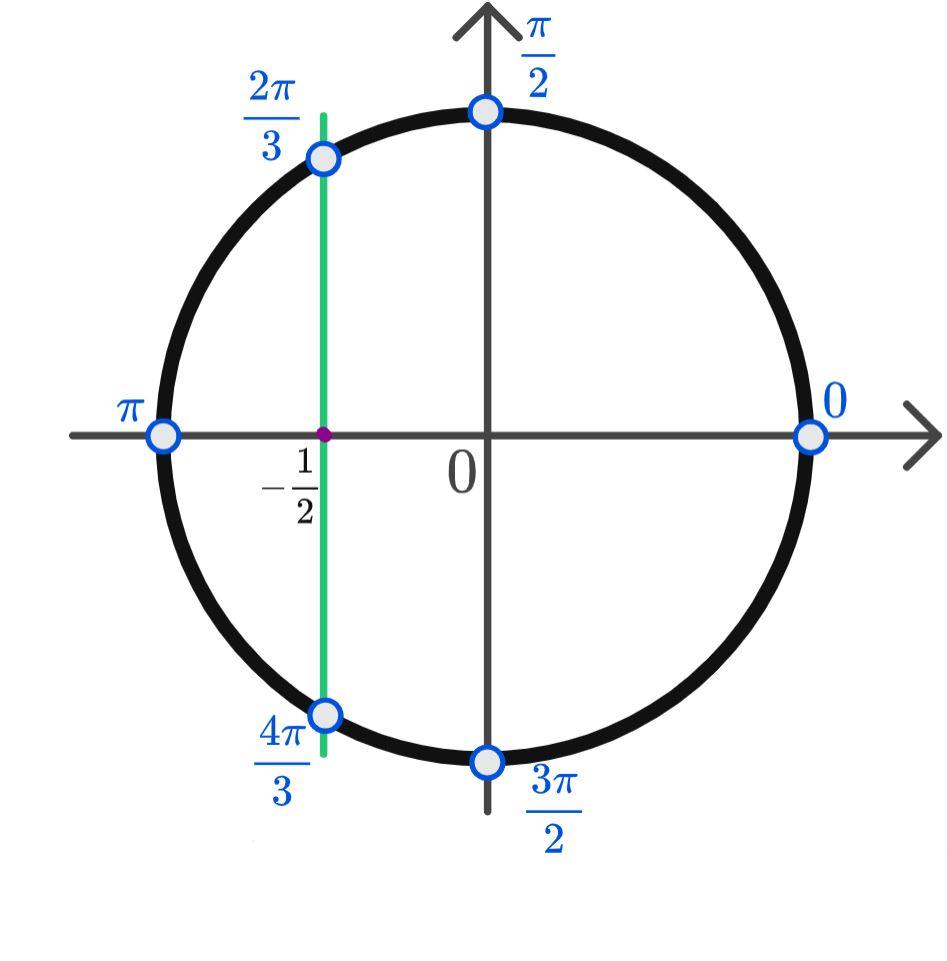
\includegraphics[width=\linewidth]{sol44}\end{figure}\end{minipage}
\end{minipage}\vspace{-9mm}\\}
{$x = \frac{\pi n}{2}$, $n\in\mathbb{Z}\,$ или $x = \pm\frac{2\pi}{3} + 2\pi n$, $n\in\mathbb{Z}$.}{Используй формулы синуса двойного и тройного углов, а затем разложи полученное выражение на множители.}
\end{problem}

\begin{problem}{Методы решения тригонометрических уравнений-2.}{10.4.7}{9D}{*}
{Известно, что $\alpha$ и $\beta$~--- острые положительные углы, для которых верна следующая система уравнений: $$\left\{
\begin{aligned}
    3\sin^{2}\alpha + 2\sin^{2}\beta&= 1\\
    3\sin 2\alpha - 2\sin 2\beta&= 0
\end{aligned}\right.$$
Показать, что угол $\alpha + 2\beta$~--- прямой (то есть $\alpha + 2\beta = \frac{\pi}{2}$).}
{НаписанноеРешение}
{ВерныйОтвет}{Подсказка}
\end{problem}

\end{document}